\chapter{Stato dell'Arte}
\label{chap:Stato dell'Arte}

\section{Risparmio energetico}
\subsection{Introduzione}
Nel settore dell'IT è ormai da parecchi anni che si guarda al problema dei consumi energetici e alle possibili soluzioni per ridurli. La tendenza verso cui questo settore sta andando è quella di spostare la parte di computazione e di storage sul Web, a carico a grandi aziende che offrono servizi di hosting o clouding. In generale ogni azienda che possiede almeno una server farm medio - grande, si dedica allo studio del risparmio energetico, in quando la spesa per l'energia per il ramo IT non è indifferente ai fini del budget aziendale. Sono stati fatti studi con lo scopo di trovare possibili soluzioni in grado di ridurre gli sprechi. Anche se non ce ne rendiamo conto, nei sistemi IT vi sono molti sprechi di energia. In \cite{ranganathan2010-pac} è illustrato che una stima del costo energetico di un Data Center di Google sia nell'ordine dei milioni di dollari per anno e che il consumo energetico del settore IT a livello mondiale sia stato stimato attorno ai 40 miliardi di dollari nel 2009. Questo fa capire come con l'evolvere della tecnologia, essa diventi sempre più potente e performante, ma necessiti anche di una quantità maggiore di energia. Per questo motivo i discorsi di consumo energetico, della riduzione degli sprechi e dell'ottimizzazione nell'uso delle risorse sono divenuti sempre più importanti e oggetto di ricerca.

\subsection{Sistemi Self-Adaptative}
 In letteratura si trovano molti studi riguardanti possibili soluzioni per una migliore gestione delle risorse e minimizzazione dello spreco di energia. Questi tipi di sistemi si chiamano Self-Adaptative, poiché riescono ad auto regolare parametri interni con l'obiettivo di consumare il minimo quantitativo di energia necessario. In applicazioni reali, bisogna però tenere conto non solo dei vincoli energetici, ma anche della qualità del servizio. E’ logico pensare che un'azienda con un data center offra servizi sul web, quindi queste soluzioni self-adaptative devono trovare un compromesso tra consumo di energia e qualità del servizio (QoS) da garantire. Questo trade-off è il motivo per cui, al giorno d'oggi, non si sono trovate soluzioni definitive. In letteratura vi sono molti articoli riguardanti sistemi auto adattativi con vincoli di QoS, come il \cite{PerezMirandolaMers2007-qosbw}, \cite{MarzollaMirandola2013-dpm}, \cite{PerezMirandolaMerseguer2014-relQoSandSWadapt} e \cite{PerezMirandolaMerseguer2014-QoSandPetriNets}. L’idea di base è di poter gestire la quantità di risorse per offrire un determinato servizio, in modo da allocarne il minor numero possibile garantendo allo stesso tempo una qualità del servizio accettabile senza che l’utente ne percepisca un degrado. Questo tipo di adattamento è ovviamente molto dinamico e molto dipendente dalla distribuzione delle richieste che vengono fatte per quel particolare servizio. Ad esempio, in \cite{PerezMirandolaMerseguer2014-QoSandPetriNets} è discussa la situazione di un server mail aziendale ed è presentato su grafico l'utilizzo del server mail nel tempo, nell'arco di una settimana. Dal grafico risulta che tra un giorno e il successivo, quindi di notte, vi è un uso limitato, mentre nella parte diurna dei giorni lavorativi si hanno alti livelli di utilizzo. Nel week-end invece un uso trascurabile. In questo caso tramite un monitoraggio, si può creare un sistema self-adaptive in grado di reagire in anticipo alle variazioni delle richieste in arrivo al server mail, allocando o deallocando risorse preventivamente. Più l'attività che si cerca di studiare non ha una distribuzione di richieste ben definita o è soggetta ad alta variabilità e magari a imprevedibili momenti di burst di richieste, più sarà difficile creare un sistema auto adattativo in grado di reagire preventivamente nel modo corretto. In questo caso lo studio del trade-off è più complicato e bisogna affidarsi a più euristiche. In generale, il concetto è di avere un sistema in grado di allocare solo le risorse necessarie a gestire l’attuale carico di lavoro col minor spreco di energia e garantendo una certa QoS. Il sistema deve anche poter anticipare un cambiamento nella frequenza di richieste in ingresso al sistema, allocando o deallocando risorse, sempre con l’obiettivo di avere attive solo le risorse necessarie a gestire il carico di lavoro.
 
 Altri esempi di più recente attualità riguardano il mondo mobile. Dall'avvento dei primi smartphone, gli utenti si sono resi subito conto che uno dei problemi di questi dispositivi è l'eccessivo consumo energetico e la conseguente poca autonomia rispetto ai cellulari della precedente generazione. Infatti, le case produttrici implementano su tutti i loro dispositivi mobili moduli di risparmio energia, in grado di agire sul sistema in base all'impostazione scelta. Anche se le impostazioni variano da brand a brand, in generale si può scegliere tra una modalità normale, senza risparmio energetico, una modalità di semi risparmio energetico e una o due modalità di super risparmio energetico in cui viene disabilitato praticamente ogni tipo di servizio non essenziale, lasciando al dispositivo le sue funzioni core e niente altro. Per quanto riguarda i dispositivi mobili ci si sta muovendo verso il Mobile Cloud Computing, come discusso in \cite{DinhLeeNiyatoWand2013-surveyMCC} . Data la potenza di elaborazione con cui sono equipaggiati i dispositivi mobili oggi giorno, essi sono a tutti gli effetti dei computer in miniatura e quindi possono fare tutto; a prova del sempre crescente numero di applicazioni create e immesse sul mercato. Tutto ciò si traduce in un consumo energetico per sostenere l'esecuzione di tutte queste applicazioni e in un problema d'immagazzinamento dati. Tramite il Mobile Cloud Computing, i dispositivi mobili posso scaricare il peso dell'elaborazione di certi dati e la memorizzazione dei file direttamente nel Cloud, con il risultato di risparmiare fino al 25\% di batteria e molto spazio di memorizzazione.
 
 Un altro ambito in cui è molto importante lo studio e l'ottimizzazione del consumo energetico è quello dell'hardware. Ad esempio nei microprocessori dei computer, ma non solo, sono presenti moduli in grado di monitorare lo stato del chip, la frequenza di lavoro e altri parametri. Nello specifico il modulo Dynamic frequency/voltage scaling (DVS) permette di regolare il voltaggio e quindi la frequenza di lavoro del processore in maniera dinamica, senza dover spegnere il componente. In \cite{MarzollaMirandola2013-dpm} sono presentate le specifiche dell’Advanced Configuration and Power Interface (ACPI) e proposte come open standard per la gestione della configurazione e dell’energia di sistemi singoli o insieme di sistemi.

\bigskip

 \section{Bluetooth 4.0 Low Energy}
 \subsection{Introduzione}
La tecnologia Bluetooth 4.0 Low Energy, nome in codice Seattle, è una tecnologia wireless ed è stata rilasciata a metà 2010, col rilascio delle le specifiche relative allo standard; ora alla versione 4.2 \cite{BT-CoreSpec4.0} . Dato un sempre maggior impiego dei dispositivi Bluetooth in svariati ambiti come l’IT, moduli di rilevamento e sensori, healtcare \cite{BT-SmartMarks} e altri ancora, questa tecnologia è stata progettata per risolvere uno dei punti deboli delle versioni precedenti: l’alto consumo energetico richiesto. Sulla tecnologia Bluetooth Low Energy, l’azienda lancia la gamma di prodotti denominati Bluetooth Smart identificando una serie di mercati in cui è richiesta una tecnologia a basso consumo energetico come le nascenti strutture delle smart home, healtcare, sport \& fitness. Questa tecnologia è stata progettata e migliorata per tutti questi dispostivi che utilizzano la batteria “a bottone” infatti, alcuni vantaggi presentati dall’azienda sono:
\begin{itemize}
	\item Basso consumo energetico.
	\item Possibile autonomia di mesi o anni per sistemi alimentati da batterie a bottone.
	\item Ampia compatibilità con molti smartphone, computer e tablet.
\end{itemize}
 Sempre nel 2010 si venne a creare un problema di retro compatibilità dei dispositivi Bluetooth Smart con tutti i dispositivi equipaggiati con tecnologie Bluetooth Classic (il Bluetooth Classic è la vecchia tecnologia dalla versione 1 fino a prima della versione 4). E’ risultato che la tecnologia Smart era completamente non compatibile con i dispositivi Bluetooth Classic. Per questo motivo nel 2011 l’azienda cambiò il logo del marchio Bluetooth Smart \cite{BT-Brand}, dividendolo in:
 \begin{itemize}
 	\item Bluetooth Smart.
 	\item Bluetooth Smart Ready.
 \end{itemize}
 L’azienda creò una versione parallela alla Smart, chiamata Smart Ready che implementa l’architettura del Bluetooth 4.0, quindi in grado di comunicare con il Bluetooth sia Smart sia Smart Ready, ma che è anche in grado di comunicare con il Bluetooth Classic, inserendo quell’elemento di retro compatibilità che mancava. Tutti i dispositivi come smartphone, computer e tablet utilizzano tecnologia Bluetooth Smart Ready, mentre dispositivi progettati per funzionare con batterie a bottone o disponibilità energetiche limitate sono equipaggiate solamente con la tecnologia Bluetooth Smart. In figura \ref{fig:bt_01} è rappresentato lo schema di compatibilità, mentre in figura \ref{fig:bt_02} è riportata la tabella di compatibilità pubblicata dall’azienda. 
 
\begin{figure}[t]
	\centering
	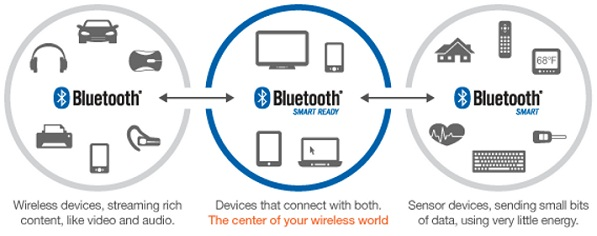
\includegraphics[width=0.9\linewidth, keepaspectratio]{Images/bt/bt_01}
	\caption[Schema di compatibilità.]{Schema di compatibilità tra dispositivi Bluetooth Classic, Smart e Smart Ready.}
	\label{fig:bt_01}
\end{figure}

\begin{figure}[ht]
	\centering
	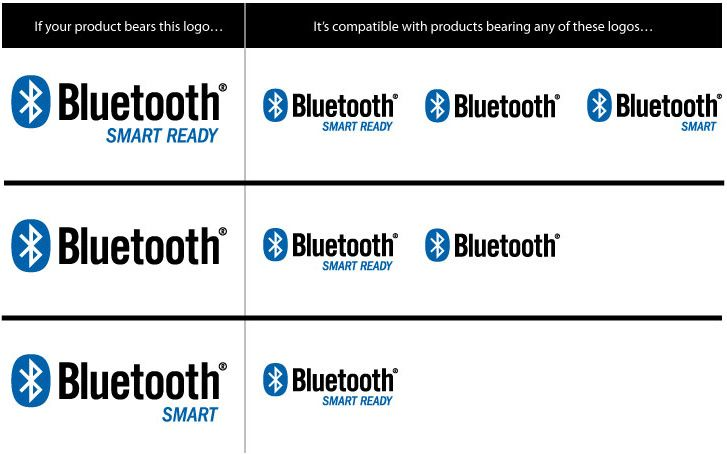
\includegraphics[width=0.9\linewidth, keepaspectratio]{Images/bt/bt_02}
	\caption[Compatibilità tecnologie]{Schema di compatibilità tra tecnologie Bluetooth}
	\label{fig:bt_02}
\end{figure}
Tutti gli smartphone, dal 2010 fino ad oggi sono stati equipaggiati con la tecnologia Low Energy Smart Ready. Si è, infatti, costatato un forte incremento nel mercato, di dispositivi che sfruttano tale tecnologia, come i bracciali con tecnologia fitbit, la serie degli i-Watch e gli smartwatch di Android che rendono l’orologio una vera e propria estensione del telefono. Tutti questi dispositivi sfruttano la tecnologia Bluetooth 4.0 Low Energy rendendo gestibile l’uso di così tante periferiche Bluetooth senza avere drammatiche conseguenze sulla durata delle batterie. Ora l’azienda Bluetooth sta già lavorando a una nuova versione del Bluetooth Low Energy, che è la versione 4.1. Essa mira a ridurre alcuni conflitti di banda con la tecnologia LTE. Infatti, la 4.0 si trova tra le bande 40 e 41 della tecnologia LTE. Per risolvere eventuali conflitti, la nuova versione 4.1 effettua un controllo di banda prima di iniziare le trasmissioni. Uno dei primi smatphone a essere equipaggiato con la nuova versione 4.1 del BLE è stato il Google Nexus 6.
\bigskip

 \subsection{Caratteristiche generali}
 
In questa sezione presentiamo, in via generale, alcune caratteristiche del Bluetooth 4.0 Low Energy, anche con qualche comparazione col predecessore Bluetooth Classic per valutare i miglioramenti e i vantaggi che questa nuova tecnologia offre.
%\vskip 3em


%\flushleft\textbf{\textit{Consumo energia}}
\subsubsection{Consumo energia}
La tecnologia Bluetooth Low Energy presenta un consumo ridotto di energia rispetto alla versione precedente, il Bluetooth Classic. Per il Bluetooth Classic vi sono tre classi distinte in cui sono categorizzati i dispositivi, con le relative distanze raggiunte e i consumi associati, mentre per il Bluetooth Low Energy, l’azienda Bluetooth non ha specificato alcun valore massimo di distanza o consumi e quindi il tutto è lasciato come libera scelta ai produttori dei trasmettitori. Questo si traduce ovviamente in una stima per il calcolo del consumo medio di questa nuova tecnologia. Nella tabella \ref{tab:carBTC} sono riportati i valori di consumi energetici e distanze, relativi al Bluetooth Classic \cite{BT-Basics}, mentre nella tabella \ref{tab:carBLE} sono riportati i valori per il Bluetooth Low Energy riportati nelle specifiche ufficiali \cite{BT-CoreSpec4.0} e anche in \cite{tesi_tibertoa2013}. Come si può vedere il consumo di energia del Low Energy è ridotto di almeno un ordine di grandezza rispetto al precedente standard Classic.

Come discusso in \cite{sensor2012}, il consumo molto basso da parte del Low Energy, permette a dispositivi alimentati con batterie a bottone, un ciclo di vita che varia tra i 2 giorni e i 14 anni. Inoltre rispetto allo standard Classic, che consente un massimo di 7 dispositivi slave per ogni master, la tecnologia Low Energy offre più flessibilità rendendo questo valore dipendente dall’applicazione e può variare tra 2 e 5.917 slave per master. Per quanto riguarda la distanza di trasmissione del Bluetooth Low Energy, è stato rilevato essere in media attorno ai 50 metri.
\bigskip
\begin{table}[h]
	\centering
	\begin{tabularx}{\textwidth}{lccc}
		\toprule
		\tableheadline{l}{} &
		\tableheadline{l}{Potenza}(mW) &
		\tableheadline{l}{Potenza}(dBm) &
		\tableheadline{l}{Distanza}(m) \\
		\midrule
		\tablefirstcol{l}{Classe 1}	& 100 & 20 & \textasciitilde100 \\
		\tablefirstcol{l}{Classe 2}	& 2.5 & 4 & \textasciitilde10 \\
		\tablefirstcol{l}{Classe 3}	& 1 & 0 & \textasciitilde1 \\
		\bottomrule
	\end{tabularx}
	\caption[Bluetooth Classic]{Caratteristiche Bluetooth Classic.}
	\label{tab:carBTC}
\end{table}
%\vskip 3em

\begin{table}[ht]
	\centering
	\begin{tabularx}{\textwidth}{ccc}
		\toprule
		\tableheadline{l}{Potenza massima} &
		\tableheadline{l}{Potenza mininima} &
		\tableheadline{l}{Distanza} \\
		\midrule
		10 mW (10 dBm) & 0.01 mW (-20 dBm) & \textasciitilde50 m \\
		\bottomrule
	\end{tabularx}
	\caption[Bluetooth Low Energy]{Caratteristiche Bluetooth Low Energy.}
	\label{tab:carBLE}
\end{table}
%\vskip 5em

\subsubsection{Link Layer}
Come descritto nelle specifiche ufficiali \cite{BT-CoreSpec4.0}, l’operatività del Link Layer può essere descritta dai seguenti stati:
\begin{itemize}
	\item Stato di Standby.
	\item Stato di Advertising.
	\item Stato di Scanning.
	\item Stato di Initiating.
	\item Stato di Connection.
\end{itemize}
Questi rappresentano i nodi dell’automa a stati finiti che modella il comportamento del Link Layer. Ogni macchina a stati può essere in un solo stato alla volta, ma un Link Layer può avere più istanze di macchina a stati, se il suo hardware lo consente. È necessario però che almeno una delle sue macchine sia in grado di entrare nello stato di Advertising o nello stato di Scanning. Nel caso di macchine a stati multiple, vi sono restrizioni sulle combinazioni possibili di stati attivi tra tutte le macchine a stati; per ulteriori dettagli si faccia riferimento alla documentazione ufficiale \cite{BT-CoreSpec4.0}.\medskip

Lo stato di Standby è uno stato in cui il dispositivo non trasmette e non riceve alcun pacchetto. Questo stato è raggiungibile da qualsiasi altro stato.\medskip

Lo stato di Advertising, trasmetterà pacchetti di advertising e, se possibile, ascolterà e risponderà a quei pacchetti trasmessi in risposta al suo pacchetto di advertising. Dispositivi nello stato di Advertising sono chiamati advertiser e lo stato di Advertising è raggiungibile dallo stato di Standby.\medskip

Lo stato di Scanning è uno stato di osservazione. Un dispositivo nello stato di Scanning rimane in ascolto per i pacchetti di advertising. Un dispositivo nello stato di Scanning è chiamato scanner e lo stato di Scanning è raggiungibile solo dallo stato di Standby.\medskip

Un Link Layer nello stato di Initiating rimarrà in ascolto per pacchetti di advertising trasmessi da determinati dispositivi e risponderà a determinati pacchetti se ha l’intenzione di aprire una connessione con quel dispositivo mittente. Un dispositivo in stato di Initiating è chiamato initiator. Lo stato di Initiating è raggiungibile dallo stato di Standby.\medskip

Lo stato di Connection può essere raggiunto sia dallo stato di Advertising sia dallo stato di Initiating. Lo stato di Connection si divide a sua volta in due ruoli:
\begin{itemize}
	\item Ruolo Master.
	\item Ruolo Slave.
\end{itemize}
Se raggiunto dallo stato di Advertising si entrerà nello stato di Connection col ruolo di Slave, mentre se si raggiunge lo stato di Connection dallo stato di Initiating si entra nello stato Connection col ruolo di Master.Un singolo dispositivo col ruolo di Slave può comunicare con un solo Master alla volta.
 
In figura \ref{fig:bt_fsa} è riportato lo schema della macchina a stati del Link Layer.
\begin{figure}[t]
	\centering
	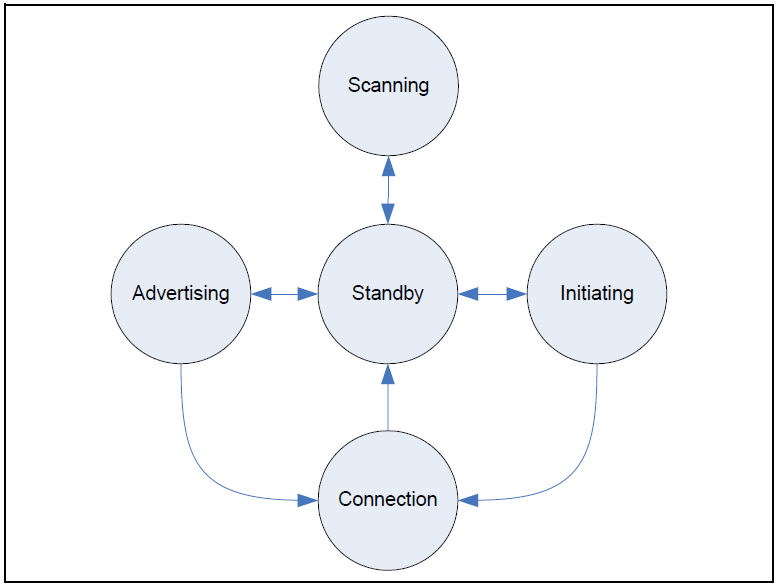
\includegraphics[width=0.9\linewidth, keepaspectratio]{Images/bt/bt_fsa}
	\caption[Schema di compatibilità.]{Schema di compatibilità tra dispositivi Bluetooth Classic, Smart e Smart Ready.}
	\label{fig:bt_fsa}
\end{figure}

\section{Reti Perr-to-Peer}
\subsection{Introduzione}
La nostra ricerca si è orientata su modelli di reti in grado di rappresentare reti Peer-to-Peer, chiamate anche Peer2Peer o P2P. Una rete P2P è una rete in cui non vi è una struttura gerarchica e ogni nodo è considerato allo stesso livello di tutti gli altri. Senza la presenza di nodi più importanti o nodi rappresentati centri di conoscenza della rete, nessun nodo può avere una visione completa della rete stessa e non può sapere se la porzione di rete da lui vista rappresenta l’intera rete. Ogni nodo quindi, ha una visione parziale e locale dell’overlay della rete. Le topologie di rete sono rappresentate da grafi bidirezionali, poiché i canali di comunicazione tra i nodi di una rete P2P per le situazioni analizzate, sono bidirezionali. Il modello di rete P2P è un’architettura logica di una rete di nodi paritari, senza alcuna struttura Client-Server fissi [\textcolor{red}{\textit{https://it.wikipedia.org/wiki/Peer-to-peer} da cambiare con il riferimento al libro !!}]; ogni nodo è paritario a tutti gli altri, infatti, ogni nodo è chiamato peer. La struttura Client-Server è creata solo nel momento di dover instaurare una connessione tra due nodi, ma più che Client-Server, sarebbe più corretto definirla come Mittente-Destinatario perché non vi sono compiti o azioni predefinite e pre-allocate nelle due parti. Può essere quindi definita una struttura particolare della struttura generica Client-Server.

La principale applicazione di questo modello di rete è stata ed è tuttora quella della condivisione dei file (file sharing), per la quale sono nati tanti sistemi quali Gnutella, FastTrak, Napster, eMule, la rete Torrent, Freenet etc.

Alcune caratteristiche delle reti Peer-to-Peer:
\begin{itemize}
	\item \textit{Basso costo d’implementazione}: non è richiesto l’uso di potenti macchine Server, ma è sufficiente che ogni peer possa sostenere le transazioni dell’utente locale e degli altri peer che vogliono connettersi a lui.
	\item \textit{Amministrazione decentralizzata}: non vi è un server centralizzato di stoccaggio delle informazioni, ma le informazioni sono in possesso dei singoli utenti, localmente, che poi mettono a disposizione della rete.
	\item \textit{Maggiore velocità di trasmissione}: non avendo un Server centralizzato cui tutti i Client si devono connettere per avere un’informazione, causando un calo nella velocità di trasferimento, in un’architettura P2P l’informazione può essere reperita anche da più nodi contemporaneamente, infatti, è possibile reperire parti diverse della stessa informazione da nodi diversi e alla fine riassemblare il tutto, col grosso vantaggio di poter avere l’informazione in tempi brevi.
	\item \textit{Sicurezza}: senza la presenza di Server centralizzati, ogni nodo deve garantire per se e per i contenuti che distribuisce, inoltre è anche esposto a ciò che riceve dalla rete che non è controllato da nessuna terza parte. 
\end{itemize}


\subsection{Modelli di Rete}
Poiché abbiamo preso in considerazione l’uso dei grafi, introduciamo due parametri riguardanti i grafi che ne descrivono alcuni aspetti. Essi sono la \textit{edge dependency} e \textit{la degree variance}.
\begin{itemize}
	\item \textbf{\textit{Edge Dependency}}: anche chiamata interdipendenza tra archi. Dato un grafo come in figura \ref{fig:edge_dependency_02}, la edge dependency è definita come la probabilità subordinata che esista un arco tra gli stati S\ped{i} \textasciitilde\: S\ped{j}, sapendo che esiste un arco tra gli stati S\ped{i} \textasciitilde\: S\ped{k} e tra S\ped{k} \textasciitilde\: S\ped{j}. Formalmente, questa probabilità si esprime così P(S\ped{i}  \textasciitilde\: S\ped{j} \textbar\: S\ped{i} \textasciitilde\: S\ped{k},S\ped{k} \textasciitilde\: S\ped{j} ) e si può considerare alta se è maggiore della sua probabilità semplice P(S\ped{i} \textasciitilde\: S\ped{j} ).
	\begin{figure}[h]
		\centering
		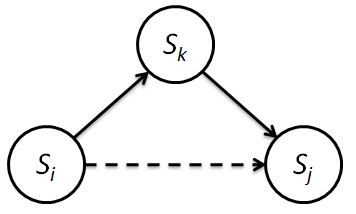
\includegraphics[width=0.7\linewidth]{Images/reti/edge_dependency_02}
		\caption[Edge dependency]{Esempio di edge dependency.}
		\label{fig:edge_dependency_02}
	\end{figure}

\end{itemize}